\chapter{Discussion of results} \label{cha:Results}

\section{Reduced complexity optimisation} \label{sec:Reduced-complexity}

In order to get an initial idea of the optimal thrust profile, a reduced complexity trajectory was modelled. This was simply implemented by deactivating secondary and tertiary perturbations, and optimising over a coarser mesh. As a result, this phase was quickly able to reach an optimal solution, giving an idea of the optimal results that would have resulted in the other phases given adequate computing power.

Most importantly, the thrust profile shown in \autoref{fig:Ascent2-thrust} demonstrates oscillations in the thrust direction between radial and tangential thrust components. This is similar to a result discovered by \textcite{Betts2003}. Unlike \textcite{Betts2003}, this is accompanied by a varying thrust magnitude, as shown in \autoref{fig:Ascent2-thrustM}. It is interesting to note that the variations in thrust magnitude are synchronous with the orbit; during the apoapsis, when thrusting is most effective in raising the periapsis, the thrust magnitude is very near to 100\%. Towards the end of the phase however, near periapsis the spacecraft often ceases thrusting altogether. The fact that thrust is continuous at the start of the phase is a result of the Oberth effect: it is most efficient to thrust when close to the central body. However, once sufficient orbital energy is attained for the periapsis to be raised beyond the van Allen belts, thrusting near periapsis contributes nothing more to achieve the objective. Thus a major objective of this study is achieved: to discover an optimal thrust profile given the thrust constraints.

\begin{figure}
\caption{Direction of thrust vector during reduced complexity ascent phase.} \label{fig:Ascent2-thrust}
\centering
\def\svgwidth{\figurewidth}
\input{Images/Ascent2/figure2.pdf_tex}
\end{figure}

\begin{figure}
\caption{Magnitude of thrust vector during reduced complexity ascent phase.} \label{fig:Ascent2-thrustM}
\centering
\def\svgwidth{\figurewidth}
\input{Images/Ascent2/figure3.pdf_tex}
\end{figure}

The resulting trajectory presents some interesting artefacts in the 3D plot at \autoref{fig:Ascent2-3D}. Once thrusting at periapsis ceases, the apoapsis stops increasing significantly. Thus the orbits are much closer together in the plot, appearing as though an inclination change has occurred.

\begin{figure}
\caption{Reduced complexity ascent trajectory in ECI frame.} \label{fig:Ascent2-3D}
\centering
\def\svgwidth{\figurewidth}
\input{Images/Ascent2/figure1.pdf_tex}
\end{figure}

%\begin{figure}
%\caption{Satellite's distance from Earth and Moon during reduced complexity ascent.} \label{fig:Ascent2-dist}
%\centering
%\def\svgwidth{\figurewidth}
%\input{Images/Ascent2/figure10.pdf_tex}
%\end{figure}
%
%\begin{figure}
%\caption{Keplerian elements of satellite within ECI frame during reduced complexity ascent phase.} \label{fig:Ascent2-kep}
%\centering
%\def\svgwidth{\figurewidth}
%\input{Images/Ascent2/figure7.pdf_tex}
%\end{figure}
%
%\begin{figure}
%\caption{Equinoctial elements of satellite within ECI frame during reduced complexity ascent phase.} \label{fig:Ascent2-mee}
%\centering
%\def\svgwidth{\figurewidth}
%\input{Images/Ascent2/figure9.pdf_tex}
%\end{figure}
%
%\begin{figure}
%\caption{Orbital energy of the satellite relative to Earth and Moon during reduced complexity ascent phase.} \label{fig:Ascent2-orbeng}
%\centering
%\def\svgwidth{\figurewidth}
%\input{Images/Ascent2/figure11.pdf_tex}
%\end{figure}
%
%\begin{figure}
%\caption{Perturbing accelerations acting on spacecraft during reduced complexity ascent phase.} \label{fig:Ascent2-pert}
%\centering
%\def\svgwidth{\figurewidth}
%\input{Images/Ascent2/figure4.pdf_tex}
%\end{figure}
%
%\begin{figure}
%\caption{Perturbing accelerations acting on spacecraft during reduced complexity ascent phase.} \label{fig:Ascent2-pert2}
%\centering
%\def\svgwidth{\figurewidth}
%\input{Images/Ascent2/figure5.pdf_tex}
%\end{figure}

The terminal condition of this phase optimisation, raising the periapsis above the van Allen belts, is shown in \autoref{fig:Ascent2-peri}. The cyclical nature of periapsis growth is due to the orbit: periapsis cannot be raised from periapsis, irrespective of the amount of thrust applied. As a result of this effect the optimised profile reduces thrust during apoapsis, conserving fuel when it is inefficient to thrust. Each of the sharp increases in periapsis corresponds to an apoapsis pass. The spacecraft's mass, seen in \autoref{fig:Ascent2-mass}, shows a steady decrease during the period of constant thrust. Then the latter half of the phase shows the results of the variable thrusting magnitude, as fuel mass is conserved at the expense of time. Consequently, this simulation used a total of 53.63~kg of ammonia, over 34.17~days. This is very close to the mission architecture's estimation of time spent in the van Allen belts, and thus corresponds to acceptable levels of radiation damage.

\begin{figure}
\caption{Periapsis of spacecraft during reduced complexity ascent phase.} \label{fig:Ascent2-peri}
\centering
\def\svgwidth{\figurewidth}
\input{Images/Ascent2/figure17.pdf_tex}
\end{figure}

\begin{figure}
\caption{Mass of spacecraft during reduced complexity ascent phase.} \label{fig:Ascent2-mass}
\centering
\def\svgwidth{\figurewidth}
\input{Images/Ascent2/figure6.pdf_tex}
\end{figure}

Finally, \autoref{fig:Ascent2-energy} shows the power levels throughout this phase. The energy used by the thrusters very closely maps the energy generated by the solar panels, until the later stages whereupon the intermittent thrusting occurs, lowering the energy requirements. Thus the constraint that the energy use does not exceed the energy generation by more than the batteries' capacity is fulfilled.

\begin{figure}
\caption{Power budget of spacecraft during reduced complexity ascent phase.} \label{fig:Ascent2-energy}
\centering
\def\svgwidth{\figurewidth}
\input{Images/Ascent2/figure16.pdf_tex}
\end{figure}

The $\Delta v$ expenditure shows a very similar profile to mass flow, albeit inverted, adding up to a total of about 1.15~kms$^{-1}$. This is very close to the expenditure estimated in the mission architecture of 1.1~kms$^{-1}$.


% Mass (6) 
% Delta-v (8)
% Phase (12)
% kep LCI (13)
% kep SEL (14)
% 3D SEL (15)

Following the reduced complexity ascent, optimisation was attempted for a reduced complexity cruise phase. However, due to the long duration of this phase and the limited computer resources available, the optimisation did not reach an optimal solution in the time available. This exercise did highlight other problems with the procedure, in particular determining a lunar capture. Due to the lunar orbit being very close to the orbital escape energy relative to the Earth (only $5\times10^5$~m$^2$s$^{-2}$), the vast majority of simulations resulted in the spacecraft escaping the Earth's sphere of influence by gaining a gravitational assist from the Moon. This caused severe computational errors as the longitude and anomaly are no longer independent parameters after escape. Another common failure scenario involved weak capture by the Moon, that is, after one or two orbits around the Moon the spacecraft would then be recaptured by the Earth. Due to the way the system was modelled, this once again caused computational errors: if the spacecraft is in orbit around the Moon in a Earth-centric frame, the anomaly becomes sinusoidal rather than always increasing; the same applies for a spacecraft in Earth orbit during a lunar-centric frame.

Determining conditions for strong lunar capture proved difficult and unreliable. Consequently it was decided to simulate the transfer backwards, from lunar orbit to Earth orbit, using an industry standard tool called Satellite Tool Kit (STK) \parencite{STK}. Backwards propagation has been used by many previous authors, such as \textcite{Kluever1995}. The main advantage to this approach is that any ascent from lunar orbit must necessarily pass through Earth orbit; whereas the reverse does not apply. Furthermore, with the Moon in a 19\degrees\ inclined orbit about the Earth, any ascent from the Moon will end up in approximately the same plane as the parking orbit after launch, thus implicitly accounting for the plane changes required to achieve the target lunar orbit. Backwards propagation is particularly well suited to this real-world application, because once the payload mass is finalised backwards propagation allows exact determination of the wet mass required.

\clearpage

%--------------------------------------------------------------------------------------------------------------------------------------------%

\section{STK modelling} \label{sec:STK}

As outlined above, the Satellite Tool Kit (STK), provided by AGI (Analytical Graphics, Inc.), was chosen to model the trajectory. STK is widely used in industry for defence and space simulation, and has developed an extensive collection of features. Recent developments have even implemented an optimiser for interplanetary trajectories. Unfortunately, STK still only supports a very limited number of optimisable parameters, for example the direction and magnitude of an impulsive burn to perform a trans-lunar injection. The high number of parameters resulting from discretisation of a continuous trajectory is, for the moment, beyond the capabilities of STK, even to the extent of solving the 2-point boundary value problem (in other words, STK cannot find a feasible solution to the problem let alone optimise it).

Therefore STK cannot target a specific orbit, such as the correct inclination and eccentricity of the GTO (after backwards propagating from LLO). However, as stated above the fact that any ascent from the Moon passes through Earth orbit, with an inclination of approximately 19\degrees\ means that it can be a very useful tool to study lunar capture. A number of simulations were performed, mostly resulting in escape orbits. However, by manipulating the start date and anomaly, it was found that some \enquote{ascents} would put the spacecraft into a stable Earth orbit (provided the thrust stops once lunar escape is achieved). From this point a geocentric frame of reference could be implemented and the PPTs could lower the orbital radius of the spacecraft relative to the Earth. Once the PPT \enquote{descent} reaches the van Allen belts for the first time, this is equivalent to the last time the spacecraft would be within the van Allen belts in the chronologically correct simulation, and consequently defines the phase boundary perfectly.

Due to the limited number of optimisable parameters, the thrust vector must be easily defined relative to one of the STK frames. For the purposes of this simulation, the thrust vector was defined to be negative velocity for the lunar phases, and positive velocity for the geocentric phases. One of the resulting trajectories is shown in \autoref{fig:STK}.

\begin{figure}
\caption{Continuous trajectory modelled in STK.} \label{fig:STK}
\centering
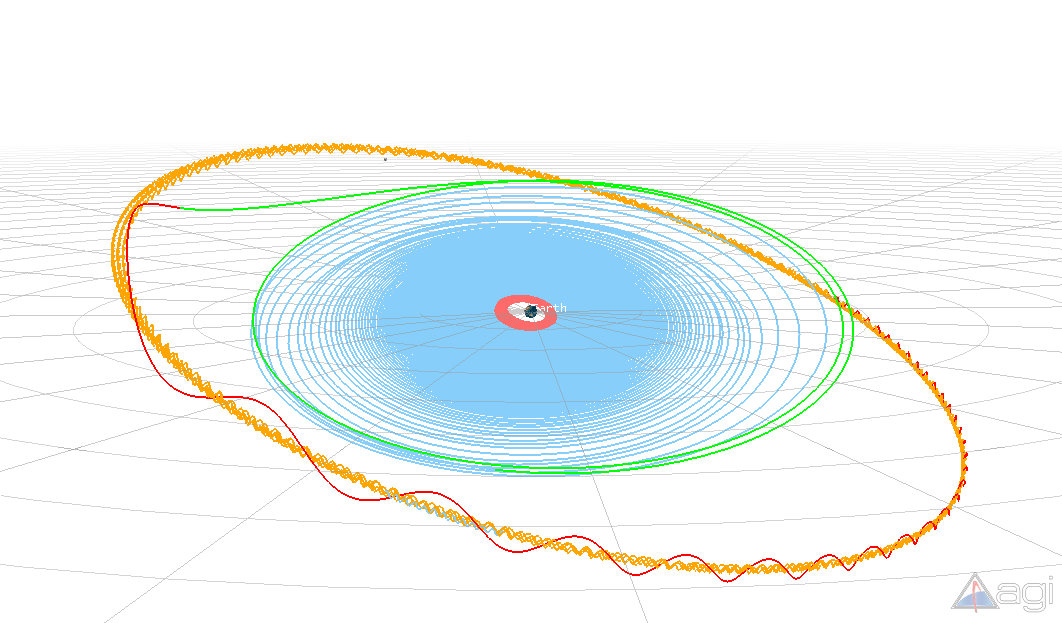
\includegraphics[width=\textwidth]{Images/STK/trajectory_white.png}
\end{figure}

Due to the inability to target specific orbits, the \enquote{descent} in STK leaves the spacecraft in the same inclination orbit it ended up in after finally escaping the Moon's gravity. The limited, predefined thrust angles mean that orbital eccentricity cannot be controlled either. Consequently the final arcjet phase was not propagated through to GTO. 

Thus the STK simulation solves the problem of lunar capture, but further work was required to determine a feasible end-to-end orbit even before any optimisation could take place. In order to manipulate the thrust profile during the forwards ascent and cruise phases such that the initial GTO could connect with the lunar capture, it was necessary to reproduce this trajectory in GESOP. 

%--------------------------------------------------------------------------------------------------------------------------------------------%

\section{Ascent} \label{sec:Ascent}
The ascent phase was modelled in GESOP subject to the initial boundary conditions outlined in \autoref{tab:Phase-2-constraints} and final boundary conditions outlined in \autoref{tab:Phase-2-3-constraints}. An initial guess was taken for the thrust profile perpendicular to the orbital radius at all times throughout ascent, in order to raise the periapsis as quickly as possible beyond the van Allen belts.

The initial guesses for starting time and mass were taken from the STK simulation. End conditions were imposed to connect this phase to the starting conditions of the cruise phase. This implementation of continuity is not ideal as it enforces an arbitrary position and velocity at the phase transitions, thus reducing the flexibility during optimisation. Ideally the phases would be optimised together, enforcing continuity between phases but not specifying what those conditions are. However this was not possible due to computational complexity, and remains an improvement for the future, perhaps exploiting parallel processing and supercomputer hardware.

Given the arbitrary nature of these continuity conditions, they were used for the initial guess but not enforced during optimisation. As the actual parameters diverged from their initial values during the optimisation, discontinuities emerged between phases. This was permitted for a number of reasons. Firstly, the launch conditions are not known, so the procedure used in this optimisation is more important than the actual result. Secondly, at every phase transition the terminating and commencing orbits are very similar, thus the variation in orbital energy was very small. In other words, the main difference between the orbits was simply timing, and at any of the phase transitions the spacecraft can sit in a parking orbit until the correct alignment occurs. Finally, due to the computational limitation of optimising each phase independently, any small change would then require all other phases to be recalculated. Treating each separately, with an implicit parking orbit in between, allows these small changes without any significant effect to the remaining phases.

\autoref{fig:Ascent-3D} shows the 3-dimensional trajectory that resulted from the ascent phase. This optimisation was able to reach a feasible solution in the computational time available, but was not allowed to continue on to find an optimal solution. Consequently the ascending orbit does not show the Oberth effect to such effect as in the reduced complexity optimisation.

\begin{figure}
\caption{Ascent trajectory in ECI frame.} \label{fig:Ascent-3D}
\centering
\def\svgwidth{\figurewidth}
\input{Images/Ascent/figure1.pdf_tex}
\end{figure}

\autoref{fig:Ascent-dist} shows the distance of the spacecraft from the Earth and Moon throughout the phase. The oscillations about the Earth are seen to slowly increase in duration and altitude, as you would expect for a slowly ascending orbit. The spacecraft's apoapsis (furthest point from the Earth) occurs with approximately the same angle as the Moon's periapsis (closest point to Earth). This is an optimal scenario, as it leads to much greater gravitational assistance earlier on in the transfer, but is unfortunately not a scenario that can be planned for, as the initial argument of periapsis is defined by the launch. The optimisation is able to imiplicitly adjust the argument of periapsis during the transfer by controlling the thrust angle, but this technique requires a lot of delta-v and therefore can only compensate for a few degrees.

\begin{figure}
\caption{Satellite's distance from Earth and Moon during ascent phase.} \label{fig:Ascent-dist}
\centering
\def\svgwidth{\figurewidth}
\input{Images/Ascent/figure10.pdf_tex}
\end{figure}

The orbital energy of the spacecraft relative to the two bodies shown in \autoref{fig:Ascent-orbeng} does not reveal much during this phase, except that the spacecraft is slowly ascending from, although still very much captured within, Earth's gravitational field. The orbital energy with respect to the Moon fluctuates as the spacecraft orbits Earth, because the gravitational potential remains relatively constant but the craft's velocity vector rotates towards the Moon and then away again. It is interesting that at times even from the GTO parking orbit, the spacecraft is very close to lunar capture ($\epsilon_m\approx0$).

\begin{figure}
\caption{Orbital energy of the satellite relative to Earth and Moon during ascent phase.} \label{fig:Ascent-orbeng}
\centering
\def\svgwidth{\figurewidth}
\input{Images/Ascent/figure11.pdf_tex}
\end{figure}

The thrust profile calculated by the optimisation is shown in \autoref{fig:Ascent-thrust}, along with the corresponding thrust magnitude in \autoref{fig:Ascent-thrustM}. While the scale of these results seems trivial, they are indicative of the direction the optimisation was pushing the solution, and suggest that the reduced complexity results form a good approximation. 

\begin{figure}
\caption{Direction of thrust vector during ascent phase.} \label{fig:Ascent-thrust}
\centering
\def\svgwidth{\figurewidth}
\input{Images/Ascent/figure2.pdf_tex}
\end{figure}

\begin{figure}
\caption{Magnitude of thrust vector during ascent phase.} \label{fig:Ascent-thrustM}
\centering
\def\svgwidth{\figurewidth}
\input{Images/Ascent/figure3.pdf_tex}
\end{figure}

\autoref{fig:Ascent-mee} shows the changing equinoctial elements of the orbit throughout the transfer, accompanied by the rather more intuitive keplerian elements in \autoref{fig:Ascent-kep}. Unsurprisingly, the semimajor axis $a$ and the semilatus rectum $p$ grow smoothly throughout the transfer, and their rate of growth increases as the spacecraft gets further from Earth's gravity well. The anomaly $\nu$ slows its growth as the orbital radius, and consequently the orbital period, increases. The spacecraft's eccentricity $e$ slowly decreases as the continual tangential thrust raises the perigee faster than the apogee, but again, this is exactly as required during this phase. The continual thrust in this phase, when compared with the optimised thrust of the reduced complexity phase, results in a higher final semimajor axis accompanied by a higher eccentricity.

\begin{figure}
\caption{Equinoctial elements of satellite within ECI frame during ascent phase.} \label{fig:Ascent-mee}
\centering
\def\svgwidth{\figurewidth}
\input{Images/Ascent/figure9.pdf_tex}
\end{figure}

\begin{figure}
\caption{Keplerian elements of satellite within ECI frame during ascent phase.} \label{fig:Ascent-kep}
\centering
\def\svgwidth{\figurewidth}
\input{Images/Ascent/figure7.pdf_tex}
\end{figure}

The stronger forces acting on the spacecraft during the ascent phase are shown in \autoref{fig:Ascent-pert}, and the weaker forces in \autoref{fig:Ascent-pert2}. It is immediately apparent that only the Earth's oblateness plays a significant role in defining the spacecraft trajectory from such a low orbit. However, as outlined in \autoref{sub:Oblateness} this only affects the argument of periapsis and right ascension of the ascending node, and therefore cannot be exploited to raise the orbit faster. As outlined above, adjusting the argument of periapsis may assist with lining up gravitational assists from the Moon later in the transfer, but due to the limitation of modelling phases separately this assist could not be incorporated. Consequently, the thrust profile was optimised purely for a fast ascent. Interestingly, the optimiser did adjust the trajectory starting date from the initial guess derived from STK, which has the effect of adjusting the phase between the spacecraft and the Moon. This shows that even the relatively weak lunar gravity present during this phase may still be exploited. The orders of magnitude between the forces shown in \autoref{fig:Ascent-pert} and the gravitational forces due to Jupiter, Venus and Mars in \autoref{fig:Ascent-pert2} highlight the reason why so many earlier studies neglect these forces. 

\begin{figure}
\caption{Perturbing accelerations acting on spacecraft during ascent phase.} \label{fig:Ascent-pert}
\centering
\def\svgwidth{\figurewidth}
\input{Images/Ascent/figure4.pdf_tex}
\end{figure}

\begin{figure}
\caption{Perturbing accelerations acting on spacecraft during ascent phase.} \label{fig:Ascent-pert2}
\centering
\def\svgwidth{\figurewidth}
\input{Images/Ascent/figure5.pdf_tex}
\end{figure}

The spacecraft periapsis is shown again in \autoref{fig:Ascent-peri}. The profile is very similar to that observed in the reduced complexity ascent, although by thrusting through the periapsis the growth is smoothed somewhat. As this is the termination condition for the phase, the final periapsis is the same between the fully optimised reduced complexity version and this one. However, the optimised phase traded off semimajor axis (and thus orbital energy) to reduce the eccentricity faster. 

\begin{figure}
\caption{Periapsis of spacecraft during ascent phase.} \label{fig:Ascent-peri}
\centering
\def\svgwidth{\figurewidth}
\input{Images/Ascent/figure17.pdf_tex}
\end{figure}

The nearly constant thrust results in fuel consumption being almost linear with time. This can be seen in \autoref{fig:Ascent-mass}, which plots the wet mass of the spacecraft over the phase. From the plot, this simulation suggested 59.82~kg worth of ammonia would be required for the ascent phase. %compare to initial guess?
Since the reduced complexity ascent, which was allowed to reach an optimal solution, took 2~days longer but saved 6~kg of ammonia propellant, a similar solution may be expected from this higher fidelity model given adequate computational power. Whether this trade off is desired is an operational decision, requiring a detailed model of solar panel degradation within the van Allen belts.

\begin{figure}
\caption{Mass of spacecraft during ascent phase.} \label{fig:Ascent-mass}
\centering
\def\svgwidth{\figurewidth}
\input{Images/Ascent/figure6.pdf_tex}
\end{figure}

\autoref{fig:Ascent-energy} shows the power generated and consumed during the phase. The energy required for the thruster demonstrates the same linear behaviour as the first half of the reduced complexity simulation, continued for the whole phase as the optimisation was not allowed to proceed to the intermittent thrust profile as the reduced complexity simulation. However, the solar panels show a much higher power generation: 1140~kWh in 32.22~days, compared to 787~kWh in 34.17~days. Given that the inclination, argument of periapsis and right ascension of the ascending node are identical to the reduced complexity ascent, and the trajectory is also very similar, there are few factors that could account for this difference. 

\begin{figure}
\caption{Power budget of spacecraft during ascent phase.} \label{fig:Ascent-energy}
\centering
\def\svgwidth{\figurewidth}
\input{Images/Ascent/figure16.pdf_tex}
\end{figure}

The biggest difference between the two simulations is the starting date: the reduced complexity phase started at the mission epoch, 1~January~2014. This simulation, based on the backwards propagated STK simulation, starts at epoch minus 140~days. In other words, this simulation starts about 4.6 months earlier than the previous one, resulting in the sun subtending a very different angle on the Earth relative to the vernal equinox. Given the constraints on pointing the solar panels towards the sun (see \autoref{sec:Vehicle-power}) this must have an affect on power generation. Since power generation has been greater than power consumption in both simulations, it does not affect the optimal trajectory, but is a factor worth investigating if more power is direct to the thrusters for a quicker ascent, as recommended in \autoref{sec:BW1-additions}.

A total $\Delta v$ of 1304~ms$^{-1}$ was expended over this phase, at an almost constant rate due to the linear thrust profile. This is rather more than the reduced complexity phase, and the $\Delta v$ estimation in the mission architecture. However, as mentioned above this sub-optimal trajectory results in a higher orbital energy than the optimised reduced complexity phase, which should decrease time and propellant needed for the subsequent cruise phase.

% In comparison, the SMART-1 ascent phase (from an initial perigee altitude of 656~km to their defined phase boundary of 20,000~km) took 1070~ms$^{-1}$ and 24~kg Xe and 1500~hours \cite{Racca9}

% DeltaV (figure8)
% Phase (figure12)
% LCI kep (figure13)
% LCI 3D (figure14)
% SEL 3D (figure15)
% Energy (figure16)

\clearpage

%--------------------------------------------------------------------------------------------------------------------------------------------%

\section{Cruise} \label{sec:Cruise}
As mentioned in \autoref{sec:Vehicle-power}, throughout the modelling and optimisation of this phase, multiple different initial guesses were trialled. Ultimately it was decided that the initial specification for vehicle performance provided the best trajectory conditions, and consequently those same parameters were used in the STK simulation mentioned in \autoref{sec:STK}. The STK trajectory was then used as an initial guess for the cruise phase, subject to boundary conditions as outlined in \autoref{sec:BVP}. Once again, for a number of reasons this phase is not continuous with preceeding or succeeding phases, but the orbital energy at the phase boundaries is very similar allowing some design flexibility.

As seen in the 3~dimensional trajectory plotted in \autoref{fig:Cruise-3D}, continual thrust leads to a circular orbit, even from a fairly elliptical starting orbit. Consequently a rendezvous with the Moon cannot really be scheduled as in previous studies involving short, higher thrust periods interspersed with coasting. Rather, lunar resonances will happen inevitably, as the spacecraft passes the Moon in its shorter, faster orbit. The purpose of optimisation therefore is to schedule the effects of these resonances, by changing the inclination or eccentricity of the spacecraft's orbit. Little work is required to achieve this, however, as all orbital changes are implicitly included in the optimisation. Of particular interest are the outermost orbits seen in the figure, whereupon the perigee is lowered (the eccentricity is increased) by a lunar assist.

\begin{figure}
\caption{Cruise trajectory in ECI frame.} \label{fig:Cruise-3D}
\centering
\def\svgwidth{\figurewidth}
\input{Images/Cruise/figure1.pdf_tex}
\end{figure}

\autoref{fig:Cruise-dist} shows the distance of the spacecraft from the Earth and the Moon over the course of the cruise phase. In comparison to the ascent phase, the spacecraft's greater distance from the Earth is apparent, resulting in greater oscillations in its distance from the Moon. The corresponding plot of orbital energies in \autoref{fig:Cruise-orbeng}, however, displays a decreasing oscillation in the spacecraft's orbital energy relative to the Moon, even as the minimum within the oscillation slowly approaches capture ($\epsilon_m\le0$). Meanwhile the orbital energy relative to the Earth approaches escape ($\epsilon_e\ge0$). 

\begin{figure}
\caption{Satellite's distance from Earth and Moon during cruise phase.} \label{fig:Cruise-dist}
\centering
\def\svgwidth{\figurewidth}
\input{Images/Cruise/figure10.pdf_tex}
\end{figure}

\begin{figure}
\caption{Orbital energy of the satellite relative to Earth and Moon during cruise phase.} \label{fig:Cruise-orbeng}
\centering
\def\svgwidth{\figurewidth}
\input{Images/Cruise/figure11.pdf_tex}
\end{figure}

The thrust profile shown in \autoref{fig:Cruise-thrust} resulted from the incomplete optimisation attempted on this phase. Despite the optimisation not having been allowed to reach an optimal solution, it is apparent that the thrust profile is once again displaying the characteristics outlined in \autoref{sec:Reduced-complexity}. It is interesting to note that the variations from purely tangential thrust seem to be directly proportional to the eccentricity, shown in \autoref{fig:Cruise-kep}, suggesting that the thrust profile is trying to circularise the orbit. Otherwise, the semimajor axis and anomaly are increasing similarly to the ascent phase.

\begin{figure}
\caption{Direction of thrust vector during cruise phase.} \label{fig:Cruise-thrust}
\centering
\def\svgwidth{\figurewidth}
\input{Images/Cruise/figure2.pdf_tex}
\end{figure}

\begin{figure}
\caption{Keplerian elements of satellite within ECI frame during cruise phase.} \label{fig:Cruise-kep}
\centering
\def\svgwidth{\figurewidth}
\input{Images/Cruise/figure7.pdf_tex}
\end{figure}

\begin{figure}
\caption{Equinoctial elements of satellite within ECI frame during cruise phase.} \label{fig:Cruise-mee}
\centering
\def\svgwidth{\figurewidth}
\input{Images/Cruise/figure9.pdf_tex}
\end{figure}

The perturbations shown in \autoref{fig:Cruise-mee} show the spacecraft thrust has dropped by two orders of magnitude, since it is now using the PPTs rather than the arcjet from the ascent phase. At the start of the cruise phase, the Earth's oblateness is still the strongest secondary force acting on the spacecraft, but this rapidly drops off as the spacecraft raises its orbit. The Moon's gravity becomes more dominant towards the end of the phase, with spikes starting to occur indicating gravitational assists caused by close passes to the Moon in the last few orbits. The sun's gravity also has a more significant effect on the spacecraft as its orbit is raised, exhibiting high frequency oscillations due to the spacecraft's orbit around the Earth, and lower frequency oscillations closely following the averaged force due to solar wind, due to the Earth's elliptical orbit around the sun.

\begin{figure}
\caption{Perturbing accelerations acting on spacecraft during cruise phase.} \label{fig:Cruise-pert}
\centering
\def\svgwidth{\figurewidth}
\input{Images/Cruise/figure4.pdf_tex}
\end{figure}

Similar cyclical behaviour is visible in \autoref{fig:Cruise-pert2}, showing the resonances of Earth's orbit with Jupiter, Venus and Mars' orbits.

\begin{figure}
\caption{Perturbing accelerations acting on spacecraft during cruise phase.} \label{fig:Cruise-pert2}
\centering
\def\svgwidth{\figurewidth}
\input{Images/Cruise/figure5.pdf_tex}
\end{figure}

Throughout the cruise phase, 17.55~kg of PTFE was consumed, generating 2519~ms$^{-1}$ of $\Delta v$. While this comprehensively demonstrates the efficacy of the PPTs compared to the arcjet used in the previous phase, the $\Delta v$ requirement was still much higher than that anticipated in the mission architecture of 1.6~kms$^{-1}$. Given the near-optimal trajectory of tangential thrust, such a large discrepancy can only be explained by an error in calculation during mission planning, or an over-estimation of the efficiency of the PPTs.

%Again for comparison, by the end of the cruise phase SMART-1 had consumed 58.8~kg Xe over 3648~hrs to generate a $\Delta v$ of 2737~ms$^{-1}$. \cite{Racca30}

% Thrust magnitude (figure3)
% Mass (figure6)
% DeltaV (figure8)
% Phase (figure12)
% LCI kep (figure13)
% LCI 3D (figure14)
% SEL 3D (figure15)
% Energy (figure16)

\clearpage 

%--------------------------------------------------------------------------------------------------------------------------------------------%

\section{Propagate} \label{sec:Propagate}

The initial mission architecture did not include a propagate phase, but during the STK simulation it was empirically found that the spacecraft achieves an appropriate orbit for lunar capture well before the Moon is in position for rendezvous. Consequently a coasting phase was inserted, when the spacecraft's trajectory was propagated forward in time without any thrusting. Given sufficient computational power, this phase could be shortened or removed entirely, much like the discontinuities between other phases, once the launch conditions are known. Whether this phase should be removed remains open to debate: it provides the spacecraft with an opportunity to recharge its batteries if the electrical system is not performing nominally, and allows time for critical adjustments if the spacecraft is drifting off course. The lunar approach is particularly important to ensure the final science phase orbit can be achieved without requiring too much propellant. Throughout this phase the spacecraft transitions from the Earth's sphere of influence to the Moon's. Consequently longitude was discarded in favour of time as the independent parameter for modelling this phase, as all the benefits outlined in \autoref{sec:Independent-parameter} are not applicable to this phase.

\autoref{fig:Propagate-3D} shows the simulated coasting trajectory. This consists of 1.5 orbits around the Earth followed by an lunar rendezvous that pulls the spacecraft into the desired lunar orbit. This orbit is apparent in \autoref{fig:Propagate-3D-lci} which plots the same trajectory but from a lunar centred frame. Since the spacecraft enters a polar orbit about the Moon, it appears to intersect the Moon given the camera is positioned above the Moon's pole. \autoref{fig:Propagate-3D-sel} shows the trajectory from the selenocentric frame, fixed relative to the Moon's surface. Because the Moon is tidally locked to the Earth, the Earth appears to be in a halo orbit in this frame.

\begin{figure}
\caption{Propagated trajectory in ECI frame. The Moon's orbit is also shown.} \label{fig:Propagate-3D}
\centering
\def\svgwidth{\figurewidth}
\input{Images/Propagate/figure1.pdf_tex}
\end{figure}

\begin{figure}
\caption{Propagated trajectory in LCI frame. The Earth's orbit is also shown.} \label{fig:Propagate-3D-lci}
\centering
\def\svgwidth{\figurewidth}
\input{Images/Propagate/figure14.pdf_tex}
\end{figure}

\begin{figure}
\caption{Propagated trajectory in SEL frame. The Earth's orbit is also shown.} \label{fig:Propagate-3D-sel}
\centering
\def\svgwidth{\figurewidth}
\input{Images/Propagate/figure15.pdf_tex}
\end{figure}

The spacecraft's distances from the Earth and the Moon are shown in \autoref{fig:Propagate-dist}. It starts on the opposite side of the Earth from the Moon, then gets pulled into lunar orbit as it swings around the Earth. 

\begin{figure}
\caption{Satellite's distance from Earth and Moon during propagate phase.} \label{fig:Propagate-dist}
\centering
\def\svgwidth{\figurewidth}
\input{Images/Propagate/figure10.pdf_tex}
\end{figure}

\autoref{fig:Propagate-orbeng} shows the corresponding orbital energies. The spacecraft has a very high orbital energy relative to the Moon whilst it is on the far side of the Earth, before being captured (dropping below $\epsilon_m=0$) towards the end of the phase. Throughout the phase the orbital energy relative to the Earth is very close to the orbital energy of the Moon relative to the Earth.

\begin{figure}
\caption{Orbital energy of the satellite relative to Earth and Moon during propagate phase.} \label{fig:Propagate-orbeng}
\centering
\def\svgwidth{\figurewidth}
\input{Images/Propagate/figure11.pdf_tex}
\end{figure}

The keplerian elements shown in \autoref{fig:Propagate-kep} show a sudden jump in semimajor axis and eccentricity as the spacecraft gets pulled towards the Moon, then another increase in semimajor axis accompanied by a drop in eccentricity as the spacecraft gets pulled into lunar orbit. The spacecraft remains at the same inclination as the Moon, but the right ascension of the ascending node ($\Omega$) is changed as the orbital plane is rotated around Earth's pole to match that of the Moon. As the spacecraft is pulled into lunar orbit, the anomaly becomes cyclical with respect to the Earth, highlighting why a lunar centric frame is necessary for the subsequent phases, and why this phase was modelled with time as the independent parameter instead of longitude, as outlined in \autoref{sec:Reduced-complexity}.

\begin{figure}
\caption{Equinoctial elements of satellite within ECI frame during propagate phase.} \label{fig:Propagate-mee}
\centering
\def\svgwidth{\figurewidth}
\input{Images/Propagate/figure9.pdf_tex}
\end{figure}

\begin{figure}
\caption{Keplerian elements of satellite within ECI frame during propagate phase.} \label{fig:Propagate-kep}
\centering
\def\svgwidth{\figurewidth}
\input{Images/Propagate/figure7.pdf_tex}
\end{figure}

\begin{figure}
\caption{Keplerian elements of satellite within LCI frame during propagate phase.} \label{fig:Propagate-kep-lci}
\centering
\def\svgwidth{\figurewidth}
\input{Images/Propagate/figure13.pdf_tex}
\end{figure}

Seen relative to the lunar frame in \autoref{fig:Propagate-kep-lci}, the semimajor axis approaches negative infinity as the spacecraft approaches capture, while the eccentricity approaches 1. At the point of capture, the spacecraft is in a parabolic orbit and the semimajor axis is undefined. As the spacecraft then descends into lunar orbit, the semimajor axis drops down from positive infinity.

\begin{figure}
\caption{Perturbing accelerations acting on spacecraft during propagate phase.} \label{fig:Propagate-pert}
\centering
\def\svgwidth{\figurewidth}
\input{Images/Propagate/figure4.pdf_tex}
\end{figure}

The perturbing forces in \autoref{fig:Propagate-pert} continue on from the previous phase, with solar and lunar gravity dominant, although there is no thrust present during this phase. As the spacecraft is descends into lunar orbit, unsurprisingly the lunar gravity becomes the dominant force. Another interesting point is the cyclical nature of the force due to Earth's oblateness that is highlighted in this plot. The sudden drops are caused when the spacecraft passes the Earth's equator, and the $J_2$ harmonic no longer has any effect on the vehicle. Furthermore, the alternating short-long-short duration between these drops is caused by the short periapsis half of the orbit, followed by the lengthy apoapsis.

%\begin{figure}
%\caption{Perturbing accelerations acting on spacecraft during propagate phase.} \label{fig:Propagate-pert2}
%\centering
%\def\svgwidth{\figurewidth}
%\input{Images/Propagate/figure5.pdf_tex}
%\end{figure}

A factor that becomes important as the spacecraft approaches capture is the angle subtended between the craft and the Moon, relative to the Earth. This is shown in \autoref{fig:Propagate-phase}. At the start of the phase, the Moon is close to its ascending node, with the spacecraft leading it by about 2 radians. As the spacecraft is in a lower, faster orbit, this angle widens until 1660 days at which point the spacecraft and the Moon are on opposite sides of the Earth. The subtended angle then approaches zero as the spacecraft approaches lunar orbit.

\begin{figure}
\caption{Longitude of spacecraft and Moon during propagate phase. The approach angle is the difference between spacecraft longitude and the Moon's longitude.} \label{fig:Propagate-phase}
\centering
\def\svgwidth{\figurewidth}
\input{Images/Propagate/figure12.pdf_tex}
\end{figure}

% Thrust direction (figure2)
% Thrust magnitude (figure3)
% Mass (figure6)
% DeltaV (figure8)
% Energy (figure16)

\clearpage

%--------------------------------------------------------------------------------------------------------------------------------------------%

\section{Capture} \label{sec:Capture}

Following the weak capture during the coasting phase propagated by the simulator the arcjet is again used, this time to lower the orbit as quickly as possible to avoid being recaptured by the Earth. This results in the spacecraft mapping increasingly small and fast circles around the Moon, as shown from the Earth's perspective in \autoref{fig:Capture-3D}.

\begin{figure}
\caption{Capture trajectory in ECI frame.} \label{fig:Capture-3D}
\centering
\def\svgwidth{\figurewidth}
\input{Images/Capture/figure1.pdf_tex}
\end{figure}

The descending spiral trajectory is far more apparent from the lunar centred frame in \autoref{fig:Capture-3D-lci}. When this frame is rotated in \autoref{fig:Capture-3D-sel} the lunar surface coverage can be seen, indicating that the science payload could be activated during this phase subject to sufficient power.

\begin{figure}
\caption{Capture trajectory in LCI frame.} \label{fig:Capture-3D-lci}
\centering
\def\svgwidth{\figurewidth}
\input{Images/Capture/figure14.pdf_tex}
\end{figure}

\begin{figure}
\caption{Capture trajectory in SEL frame viewed from Moon's pole.} \label{fig:Capture-3D-sel}
\centering
\def\svgwidth{\figurewidth}
\input{Images/Capture/figure15.pdf_tex}
\end{figure}

%\begin{figure}
%\centering
%\def\svgwidth{\figurewidth}
%\input{Images/Capture/3D-sel-side.pdf}
%\caption{Capture trajectory in SEL frame viewed from Moon's equator.} \label{fig:Capture-3D-sel-side}
%\end{figure}

The satellite's distance from the respective bodies in \autoref{fig:Capture-dist} is unsurprising: it gets closer to the Moon, while its orbit about the Moon causes oscillations in the distance to Earth that approach the Earth-Moon distance as the orbit descends. The orbital energy plot in \autoref{fig:Capture-orbeng} is more interesting, showing the spacecraft's precariously captured lunar orbit becoming more stable. Meanwhile, the orbital energy with respect to the Earth starts oscillating wildly. The spacecraft's gravitational potential with respect to the Earth is more or less constant, so the oscillations are caused by the velocity vector oscillating towards and then away from the Earth. A consequence of this is that when the spacecraft's velocity is directed away from the Earth, it exceeds escape velocity, so the orbital energy is positive. If not for the Moon repeatedly pulling the spacecraft back again, it would escape the Earth's gravity field.

\begin{figure}
\caption{Satellite's distance from Earth and Moon during capture phase.} \label{fig:Capture-dist}
\centering
\def\svgwidth{\figurewidth}
\input{Images/Capture/figure10.pdf_tex}
\end{figure}

\begin{figure}
\centering
\def\svgwidth{\figurewidth}
\input{Images/Capture/figure11.pdf_tex}
\caption{Orbital energy of the satellite relative to Earth and Moon during capture phase.} \label{fig:Capture-orbeng}
\end{figure}

During the capture phase, the semimajor axis steadily decreases very similar to the ascent phase in reverse. Similarly, the anomaly increases at an increasing rate, and the lower orbit results in higher orbital speed. Unlike a reversed descent phase, the eccentricity continues to decrease until it reaches a very nearly circular orbit, as required for the science phase. For the first half of the phase, the argument of periapsis is increasing while the anomaly is almost steady. This has essentially the same effect as the anomaly increasing, since the orbit is almost circular. The right ascension of the ascending node precesses steadily as a result of the Earth's gravity, a well known phenomenon of polar lunar orbits \parencite{Gupta2011}. % BULLSHIT?

\begin{figure}
\centering
\def\svgwidth{\figurewidth}
\input{Images/Capture/figure13.pdf_tex}
\caption{Keplerian elements of satellite within LCI frame during capture phase.} \label{fig:Capture-kep-lci}
\end{figure}

\begin{figure}
\centering
\def\svgwidth{\figurewidth}
\input{Images/Capture/figure9.pdf_tex}
\caption{Equinoctial elements of satellite within LCI frame during capture phase.} \label{fig:Capture-mee}
\end{figure}

In the plot of perturbations acting on the spacecraft over the capture phase, shown in \autoref{fig:Capture-pert}, the acceleration due to spacecraft thrust is observed to slowly increase. This is because propellant is expelled as the spacecraft thrusts, thereby reducing the mass being accelerated. This phenomenon is present in every powered phase, but is most apparent during the capture phase because the arcjet is in use, resulting in a higher mass flux than the descent phase, combined with the lighter load than previous phases because much of the fuel has already been used.

The Earth's gravity continues to decrease in effect as the spacecraft settles to a steady distance from the Earth, but the perturbations due to the Moon's oblateness rapidly increase in magnitude. 

\begin{figure}
\centering
\def\svgwidth{\figurewidth}
\input{Images/Capture/figure4.pdf_tex}
\caption{Perturbing accelerations acting on spacecraft during capture phase.} \label{fig:Capture-pert}
\end{figure}

\begin{figure}
\centering
\def\svgwidth{\figurewidth}
\input{Images/Capture/figure5.pdf_tex}
\caption{Perturbing accelerations acting on spacecraft during capture phase.} \label{fig:Capture-pert2}
\end{figure}

\autoref{fig:Capture-thrust} shows the thrust profile resulting from the capture phase simulation. This profile results from the initial guess, of continual thrust backwards along the velocity vector. Consequently the thrust initially has a substantial radial component due to the eccentricity of the orbit, but rapidly settles into almost purely tangential thrust. The noise in the out-of-plane component results from truncation error when evaluating the unit thrust vector constraint.

\begin{figure}
\centering
\def\svgwidth{\figurewidth}
\input{Images/Capture/figure2.pdf_tex}
\caption{Direction of thrust vector during capture phase.} \label{fig:Capture-thrust}
\end{figure}

Over the course of the capture phase, 33.43~kg of ammonia propellant was used. This generated almost 968~ms$^{-1}$ of $\Delta v$, compared to the mission architecture guess of 0.5~kms$^{-1}$. Once again this is a substantial difference that is unlikely to be accounted for by allowing the phase optimisation to reach an optimal solution. It is more likely that if the entire multiple-phase trajectory were optimised together, a substantial saving in $\Delta v$ could be achieved (and correspondingly fuel consumption) particularly in the troublesome area of lunar capture, as the optimiser would be able to evaluate different capture scenarios. However, the mission architecture estimates were based on a low-fidelity STK simulation, and as such is unlikely to have investigated complex lunar capture techniques. Consequently it must be concluded that the initial estimates were optimistic.


% Thrust direction (figure2)
% Thrust magnitude (figure3)
% Mass (figure6)
% ECI kep (figure7)
% DeltaV (figure8)
% Phase (figure12)
% Energy (figure16)

\clearpage

%--------------------------------------------------------------------------------------------------------------------------------------------%

\section{Descent} \label{sec:Descent}

\autoref{fig:Descent-3D-lci} shows the descent phase trajectory in an inertial lunar centred frame. The terminal conditions of the capture phase are propagated to the science orbit using the PPTs. This results in the very tight, very nearly circular spiral seen in the figure.

\begin{figure}
\centering
\def\svgwidth{\figurewidth}
\input{Images/Descent/figure14.pdf_tex}
\caption{Descent trajectory in LCI frame.} \label{fig:Descent-3D-lci}
\end{figure}

In the rotating surface-fixed frame of \autoref{fig:Descent-3D-sel}, the slow decrease in orbital altitude can be seen.

\begin{figure}
\centering
\def\svgwidth{\figurewidth}
\input{Images/Descent/figure15.pdf_tex}
\caption{Descent trajectory in SEL frame.} \label{fig:Descent-3D-sel}
\end{figure}

The spacecraft's distance from the Earth and the Moon is almost trivial during this phase: the distance from the Moon decreases gradually, but on the plot this change is overwhelmed by the distance from the Earth, which closely maps the distance of the Earth from the Moon.

\begin{figure}
\centering
\def\svgwidth{\figurewidth}
\input{Images/Descent/figure10.pdf_tex}
\caption{Satellite's distance from Earth and Moon during descent phase.} \label{fig:Descent-dist}
\end{figure}

A more interesting artefact emerges in the plot of orbital energy seen in \autoref{fig:Descent-orbeng}. The spacecraft's orbital energy relative to the Earth oscillates as described in \autoref{sec:Capture}, but since the spacecraft is in a nearly polar orbit twice in every orbit the Moon makes around the Earth the spacecraft's orbit becomes perpendicular to the Earth-Moon vector. Consequently the amplitude of this oscillation also oscillates. As the spacecraft gets closer to the Moon, its velocity increases, and its orbital energy relative to the Earth rises further beyond escape velocity.

\begin{figure}
\centering
\def\svgwidth{\figurewidth}
\input{Images/Descent/figure11.pdf_tex}
\caption{Orbital energy of the satellite relative to Earth and Moon during descent phase.} \label{fig:Descent-orbeng}
\end{figure}

Throughout the phase, the semimajor axis steadily drops as desired, while the eccentricity has already started a small but inexorable increase due to the lunar mascons that will ultimately cause the spacecraft to crash into the surface. The right ascension continues to precess.

\begin{figure}
\centering
\def\svgwidth{\figurewidth}
\input{Images/Descent/figure13.pdf_tex}
\caption{Keplerian elements of satellite within LCI frame during descent phase.} \label{fig:Descent-kep-lci}
\end{figure}

\begin{figure}
\centering
\def\svgwidth{\figurewidth}
\input{Images/Descent/figure9.pdf_tex}
\caption{Equinoctial elements of satellite within LCI frame during descent phase.} \label{fig:Descent-mee}
\end{figure}

In the plots of perturbing forces acting on the spacecraft during the descent phase (\autoref{fig:Descent-pert} and \autoref{fig:Descent-pert2}), the Earth's orbit about the Sun is once again apparent in the solar gravity and solar wind. Forces due to the Moon's gravitational harmonics are increasing in strength as the craft gets closer to the surface, but the dominant secondary force is still Earth's gravity.

\begin{figure}
\centering
\def\svgwidth{\figurewidth}
\input{Images/Descent/figure4.pdf_tex}
\caption{Perturbing accelerations acting on spacecraft during descent phase.} \label{fig:Descent-pert}
\end{figure}

\begin{figure}
\centering
\def\svgwidth{\figurewidth}
\input{Images/Descent/figure5.pdf_tex}
\caption{Perturbing accelerations acting on spacecraft during descent phase.} \label{fig:Descent-pert2}
\end{figure}

The thrust throughout the descent phase is directed backwards along the velocity vector. Since the orbit is very nearly circular, this thrust is primarily tangential to the circle being described, with very small radial components. Once again the out-of-plane thrust is a negligible truncation error.

\begin{figure}
\centering
\def\svgwidth{\figurewidth}
\input{Images/Descent/figure2.pdf_tex}
\caption{Direction of thrust vector during descent phase.} \label{fig:Descent-thrust}
\end{figure}

The simulation of this phase estimated 1.43~kg PTFE was consumed, providing almost 390~ms$^{-1}$. This $\Delta v$ is almost exactly as estimated in the mission architecture. Once again the PPTs are remarkably efficient for a phase that lasted 91.79~days. As with the cruise phase, there is a surplus of energy available, although the power generation slows late in the phase as the spacecraft begins transiting through the Moon's shadow.

% ECI 3D (figure1)
% Thrust magnitude (figure3)
% Mass (figure6)
% ECI kep (figure7)
% DeltaV (figure8)
% Phase (figure12)
% Energy (figure16)

\clearpage

%--------------------------------------------------------------------------------------------------------------------------------------------%

\section{Science} \label{sec:Science}

As there is no propulsive thrust during the science phase, the orbit was propagated forwards for 6 months to determine the spacecraft's behaviour in the absence of stationkeeping manoeuvres. \autoref{fig:Science-3D-lci} shows the final orbit in an inertial frame. The surface coverage is shown in \autoref{fig:Science-3D-sel}: the whole Moon's surface covered repeatedly within the 6 month period. 

\begin{figure}
\centering
\def\svgwidth{\figurewidth}
\input{Images/Science/figure14.pdf_tex}
\caption{Science trajectory in LCI frame.} \label{fig:Science-3D-lci}
\end{figure}

\begin{figure}
\centering
\def\svgwidth{\figurewidth}
\input{Images/Science/figure15.pdf_tex}
\caption{Science trajectory in SEL frame.} \label{fig:Science-3D-sel}
\end{figure}

The keplerian elements shown in \autoref{fig:Science-kep-lci} shows oscillations in the semimajor axis caused by the mascons. More worryingly, the eccentricity shows a steady increase throughout the phase, indicating an increasingly elliptical orbit that would eventually cause the spacecraft to impact the Moon's surface. This trend is more visibly seen in \autoref{fig:Science-peri}, showing the resultant decrease in periapsis radius. On the other hand, the sudden change in argument of periapsis ($\omega$) towards the start of the phase holds little meaning as the orbit is almost circular at that point. The right ascension of the ascending node contines to precess. These behaviours all resemble the 130~km lunar orbit modelled by \textcite{Gupta2011} very closely.

\begin{figure}
\centering
\def\svgwidth{\figurewidth}
\input{Images/Science/figure13.pdf_tex}
\caption{Keplerian elements of satellite within LCI frame during science phase.} \label{fig:Science-kep-lci}
\end{figure}

\begin{figure}
\centering
\def\svgwidth{\figurewidth}
\input{Images/Science/figure9.pdf_tex}
\caption{Equinoctial elements of satellite within ECI frame during science phase.} \label{fig:Science-mee}
\end{figure}

\begin{figure}
\centering
\def\svgwidth{\figurewidth}
\input{Images/Science/figure17.pdf_tex}
\caption{Periapsis of spacecraft during science phase.} \label{fig:Science-peri}
\end{figure}

\begin{figure}
\centering
\def\svgwidth{\figurewidth}
\input{Images/Science/figure4.pdf_tex}
\caption{Perturbing accelerations acting on spacecraft during science phase.} \label{fig:Science-pert}
\end{figure}

%\begin{figure}
%\centering
%\def\svgwidth{\figurewidth}
%\input{Images/Science/figure5.pdf_tex}
%\caption{Perturbing accelerations acting on spacecraft during science phase.} \label{fig:Science-pert2}
%\end{figure}

% ECI 3D (figure1)
% Thrust direction (figure2)
% Thrust magnitude (figure3)
% Mass (figure6)
% ECI kep (figure7)
% DeltaV (figure8)
% Distances (figure10)
% Orbital energy (figure11)
% Phase (figure12)
% Energy (figure16)

\clearpage

%--------------------------------------------------------------------------------------------------------------------------------------------%

\section{Validation} \label{sec:Validation}
For obvious reasons there have been few experimental flights to validate low-thrust trajectory theory, and no flight testing is possible to verify this particular proposed trajectory prior to final launch. However, the laws governing forces acting on spacecraft are known better than other theory, for example atmospheric trajectories. 

The mechanics outlined in \autoref{cha:Orbital-dynamics-and-modelling} have been well established for many decades \parencite{Kaplan1976}, but were further verified in Matlab prior to commencing work with GESOP. The optimisation routines within GESOP, and the flight mechanics of ASTOS, have been numerically verified by ESTEC, Dassault, Astrium, CNES, EADS and JAXA, among other industrial partners. It is practically validated by ongoing use on real missions launched by ESA and DLR, including Ariane 5 and Vega rocket launches, the ExoMars and Beagle 2 missions, and X38 re-entry scenarios.

The independently computed phases from GESOP are plotted together in \autoref{fig:Whole-trajectory}. Note that this is merely conceptual; the temporal discontinuities between phases require parking orbits be inserted, or else the trajectories be revised. Once launch data is known, the complete trajectory may be calculated. Nonetheless, it is worth comparing the trajectory to \autoref{fig:STK} for a qualitative analysis that orbital energy is conserved.

\begin{figure}
\centering
\def\svgwidth{0.8\textwidth}
\input{Images/figure0.pdf_tex}
\caption{The complete GESOP trajectory.} \label{fig:Whole-trajectory}
\end{figure}

For the purposes of further validation, the control vector profile developed in GESOP was converted into quaternions using Matlab, and then combined with the Ephemeris Time to fit the specifications for STK external attitude files. A generic scenario was then produced in STK using the external attitude files along with thruster specifications and phase lengths identical to those used in GESOP with a high precision propagator, resulting in the trajectories as seen in \autoref{fig:STK-verification-ascent}, \autoref{fig:STK-verification-cruise}, \autoref{fig:STK-verification-capture}, and \autoref{fig:STK-verification-descent}.

\begin{figure}
\centering
\includegraphics[width=0.8\textwidth]{Images/STK/ascent.png}
\caption{STK validation of ascent phase.} \label{fig:STK-verification-ascent}
\end{figure}


\begin{figure}
\centering
\includegraphics[width=0.8\textwidth]{Images/STK/cruise.png}
\caption{STK validation of cruise phase.} \label{fig:STK-verification-cruise}
\end{figure}


\begin{figure}
\centering
\includegraphics[width=0.8\textwidth]{Images/STK/capture.png}
\caption{STK validation of capture phase.} \label{fig:STK-verification-capture}
\end{figure}


\begin{figure}
\centering
\includegraphics[width=0.8\textwidth]{Images/STK/descent.png}
\caption{STK validation of descent phase.} \label{fig:STK-verification-descent}
\end{figure}

There were minor differences %as seen in \autoref{fig:STK-verification}
due to different orders of accuracy in Earth oblateness and the algorithms used to calculate third body perturbations, but these differences were negligible in most cases% as seen in \autoref{fig:STK-error}
. \autoref{fig:STK-verification-capture} does highlight the importance of updating the trajectory during flight; due to these minor numerical differences, the thrust profile gets slightly out of synchrony with the orbit. Consequently, instead of approaching a low, circular lunar orbit the argument of periapsis starts precess and the eccentricity increases, until the trajectory intersects the Moon's surface. This problem could be avoided by monitoring the spacecraft's position from the ground, and periodically uploading a revised thrust profile to the craft.

%\begin{figure}
%\centering
%%\includegraphics{}
%\caption{STK validation modelling.} \label{fig:STK-verification}
%\end{figure}
%
%\begin{figure}
%\centering
%%\includegraphics{}
%\caption{Difference between STK modelling and GESOP modelling.} \label{fig:STK-error}
%\end{figure}

While this trajectory simulation cannot verify that the solution is optimal, it does confirm that the solution is feasible, and can be used to compare trajectories on a case-by-case basis. For example, this trajectory required 93.25~kg of ammonia propellant for the arcjet over the ascent and capture phases, and 18.98~kg of PTFE propellant for the PPTs over the cruise and descent phases. In comparison, SMART-1 used 82~kg of xenon propellant to complete a similar trajectory \parencite{Estublier2007}. This discrepancy suggests that despite the efficiency of the PPT thrusters, the fuel efficiency and average $I_{sp}$ of \BW\ are severely compromised by excessive use of the thermal arcjet. It is assumed that should sufficient computational power allow the entire trajectory be optimised as a whole, arcjet phases would be reduced and PPT phases extended to reduce the total propellant consumption.

%59.82~kg ammonia on the ascent phase over 32.22~days
%6~kg less for reduced complexity ascent (10\% saving) but took 2 days longer
%17.55~kg PTFE during cruise phase over 1123.91~days
%33.43~kg ammonia during capture phase over 18~days
%1.43~kg PTFE during descent phase over 91.791~days

% Comparison SMART-1 \cite{Estublier2002} 82~kg Xe 4958~hours thrust 1540~s average Isp 3.7~kms$^{-1}$ total delta-V (74~kg and 3.5~kms$^{-1}$ before stationkeeping)

The fully optimised but lower complexity ascent phase verifies that this optimisation process does improve the propellant consumption. When the computational cycle was allowed to finish, the new trajectory required 6~kg less propellant at the expense of 2~days longer phase duration. This represents a 10\% improvement over the phase. While the subsequent phases are too different to assume a similar improvement, further exploitation of lunar gravitational assists and the Oberth effect will improve the fuel efficiency.

Failed optimisation runs demonstrate the resilience of the optimisation process. For example, one optimisation run for the reduced complexity ascent phase inadvertently neglected to constrain the starting mass. The optimiser subsequently maximised the final mass by increasing the starting mass up to the hard limit set by the parameter bounds (see \autoref{sub:Scaling}). While this optimisation took 6~days to complete due to the chaotic solution space, the fact that the optimiser was able to incrementally adjust the starting mass all the way to the hard limit demonstrates a surprising tolerance for a stiff, chaotic solution space.

%Optimisation run from 15/4/2011 to 21/4/2011. neglected to constrain mass starting value for ascent phase. optimiser found best way to maximise final mass was to increase the initial mass as far as possible (hard limit set by parameter bounds for affine transform). suggests a continuous optimisation to higher mass. computation took so long perhaps because the entire trajectory changed every time the mass changed? just VAB escape so minor changes probably less significant than later on (closer to moon). Less stiff problem.

Finally, the trajectory will receive ultimate verification when satellite is launched. Unfortunately at this stage in the design, there is still no fixed launch date scheduled.





\section{Summary} \label{sec:Results-summary}

Results have been presented for a reduced complexity ascent phase that was able to find an optimal solution, followed by a high fidelity ascent phase that was stopped after finding a feasible solution. A partially optimised cruise phase was then presented, followed by the subsequent capture, descent and science phases. The initial guess was derived from an STK backwards propagation model which is also described.

These results do not constitute a complete trajectory due to the absence of important mission data such as launch date and spacecraft payload mass. However, a robust trajectory design procedure is demonstrated with indicative results to aid in refining the mission architecture. 

